\graphicspath{{images/}}

\section{\thesection~Discussion}
\label{sec:discussion}

Fits of the competition model (see Figures~\ref{fig:comp_fit_plate}
and \ref{fig:comp_fit_zone}) use less parameters and are qualitatively
better than fits of either the logistic or generalised logistic model
from the QFA R package \citep{Addinall2011,qfa2016}. Competition model
ranking of growth estimates for repeats on P15 (see
Figure~\ref{fig:comp_vs_log_ranking}) agree with the logistic model
rankings from \citet{Addinall2011} for the fastest and slowest growers
(and with rankings from independent spot tests (refs) CHECK
THIS). However, there is much disagreement in the rank of other
strains. (Could also do with the correlation plot for P15). The
reliability of growth estimates was not improved using the competition
model for the fastest growing strains on P15 (see
Figure~\ref{fig:comp_b_log_r_cov}). This may be due to the effect of
noise dominated cell observations from slow growing cultures on
collectively fit parameters. This did not affect the the logistic
model which fit to cultures individual. The greater reliability of
estimates for slow growing cultures could be entirely due to
collective fitting rather than to correcting for competition. (Could
do with p-values on figure; also bold HIS3 everywhere) Unfortunately,
the change in order for middle rankings is unlikely to identify new
genetic interactions because significance is determined by comparison
to a neutral deletion also in this range. Although improved,
uncertainty in estimates for the slowest growers is still much higher
than for the fastest meaning that the power to infer genetic reactions
is not dramatically improved. (HIS3 has about half the variance for
the competition model and this could be
significant.)

Fitting the logistic model to slower growing cultures requires
heuristic checks to correct for confounding between \(r\) and
\(K\). The QFA R implementation appears to have some issues. The
strains \textit{est1\(\Delta\)} and \textit{rad50\(\Delta\)} have
dramatic changes in ranking between logistic model \(r\) and \(MDR\)
(see Figure~\ref{fig:comp_vs_log_ranking}). In independent spot tests
(ref) these are very sick strains and I confirmed this in the raw QFA
images by visual inspection. High \(r\) and low \(K\) have been
erroneously fit to both strains. This is corrected for when converting
to \(MDR\) which agrees with the competition model ranking and
independent validation and is more similar to the fitness measure
(\(MDR \times MDP\)) used in the original analysis by
\citet{Addinall2011}. For other cultures it appears that encroachment
of fast growing cultures into neighbours is affecting cell density
estimates made by Colonyzer \citep{Lawless2010}. In logistic fits some
growth curves are still in the exponential phase at the end of
observations and this may be another fitting issue. If repeated, the
plate from \citet{Addinall2011} should be run with a lower
concentration of nutrients in the agar so that the stationary phase
can be reached before cultures start to merge.

I looked at plate images from QFA and Colonyzer to investigate other
discrepancies.~\textit{mre11\(\Delta\)} is a weak growing strain (ref
validation) which was misclassified as healthy by the competition
model but not the logistic model. One repeat contained unusual
heterogeneity, which may be natural or the results of contamination,
and may explain the discrepancy. (Should take median value next
time). \textit{hap4\(\Delta\)} appears to be much healthier
than \textit{zrt3\(\Delta\)} which agrees with the competition model
but not the logistic model. Although the precision of estimates is
similar for both models, the competition model appears to be more
accurate. Unfortunately, I lack independent data for validation of the
middle strains.

Recent work Herrmann and Lawless suggests that direct measures of
\(C(0)\) may not be reliable due to heterogeneity between cells
in the same inoculum; many cells do not grow and only the fastest
growing cells contribute significantly to the final population. A
plate level \(C(0)\) also seems inappropriate but having extra
parameters for the staring cell density of each culture is
undesirable. Only a small amount of nutrients is used when cultures
are small. Therefore, cultures could be grown for a short time before
making direct cell density measurements that may be more accurate. QFA
inocula use cells taken from the stationary phase where there might be
more heterogeneity (ref). It may be possible to increase the
reliability of fitness estimates by taking inocula from the
exponential growth phase or using a higher starting density to average
out effects.

The Stripes and Filled plates used a higher inoculum density and had
very few noise-dominated cultures. Compared to P15, this would have
reduced noise in collectively fit competition model estimates and
would not have required heuristic checks to be employed for the
logistic model. This may therefore be a fairer comparison than
P15. Correlation of fitness estimates between plates in
Figure~\ref{fig:}a was similar for both models. This is despite not
finding global minima with the competition model. However, correlation
between models for the same plate in Figure~\ref{fig:r_correlations}b
is poor. (Could definitely do with P15 correlations to compare). There
are issues with validation for both models (see
Figure~\ref{fig:stripes_validation}); the logistic model does not
account for differences between plates at all and the competition
model overcorrects. As I lack independent data for validation it is
difficult to decide which to believe. (Unfortunately, these plates
lack repeats so I could not study the reliability of estimates on the
same plate. (I believe that we have more issues with accuracy than
precision anyway). It would be informative to repeat P15 with
\(C(0)\) at a measurable level. In any case, it is clear that the
competition model could be improved.


\subsection{\thesubsection~Future work}

I was unable to find global minima using a gradient method (see
Section~\ref{sec:fitting_comp}) to fit the competition model. I began
work on a genetic algorithm method of solving but lacked time to
complete this. I did however find that, with fixed plate level
parameters, it is possible to reliably return \(b_{i}\) with a
gradient method (see Figure~\ref{fig:comp_fit_fixed_plate_level}. This
offers the potential to use a hierarchical genetic algorithm where
candidate plate level parameters are fixed in gradient fits of culture
level parameters. Alternatively, a pure hierarchical genetic algorithm
may work (i.e. where \(b_{i}\) are also evolved). A hierarchical
Bayesian approach to fitting the competition model, similar to that of
\citet{Heydari2016} for the logistic model, could also return global
minima but might be slow. Current best fits, which are different local
minima, have well correlated fitness rankings and make similar
overcorrections for competition. This suggests that there is a more
fundamental issue with the model.

It would be informative to validate the independent limit of the
competition model to determine whether a mass action approximation is
valid and whether it is correct to ignore the effect of metabolism on
nutrient and final cell density. I suggest to validate first in liquid
cultures, where the assumption of a well stirred mixture is more
valid, and then attempt to validate for single cultures grown on agar,
which more closely resembles QFA. Growth on a surface has a lower
dimensionality and may be diffusion limited so a fractal kinetics
model may be required \citep{Kopelman1988,savageau1995}. Nutrients
(sugars, nitrogen, etc.) in QFA agars are of a standard composition,
designed to reduce the excess of any single nutrient (check QFA paper
and cite). It would be helpful to know and control the identity of the
limiting nutrient using a different formula of agar. With nitrogen,
rather than sugar, as the limiting nutrient, we are less likely to
have to model metabolism.


Estimates of the nutrient diffusion constant \(k_{n}\) were fairly
high such that nutrients diffused readily between neighbours and were
nearly depleted when growth stopped. It may be that growth becomes
limited by the diffusion of nutrients through agar before all
nutrients are depleted and that nutrients are not well approximated as
being evenly distributed withing the spatial scales that we
model. Using a finer grid could reduce the overcorrection seen in
Figure~\ref{fig:stripes_validation}. \citet{Reo2014} use the diffusion
equation (with Neumann and Dirichlet boundary conditions) to simulate
nutrient dependent growth of a single bacterial culture on a pertri
dish in two-dimensions. They create a sink for nutrients from culture
growth and equate the flux of nutrients through culture area with the
rate of increase in culture size. They model culture area as varying
and keep culture density constant. This model could be adapted for QFA
by keeping culture area constant and allowing culture density to
vary. A mass action kinetic model of reaction~(\ref{eq:reaction})
could be used for culture growth and the nutrient sink. It is
computationally unfeasible to use such a detailed model to fit a whole
plate but simulation could be very informative.

If we find that competition for nutrients is not responsible for the
interaction between neighbours, for instance if growth becomes limited
by diffusion of nutrients in the agar before nutrients from neighbours
can be accessed, then we could instead model signalling by ethanol
poisoning. This may be modelled similarly to how the competition model
models nutrient diffusion and much of the code could be reused.
(Quorum sensing via the molecule amonia could also be having an effect
(ref)). If there is any combination of competition, metabolism,
signalling, or arrest contributing significantly to differences in the
growth of cultures and the interaction between neighbours then it will
be difficult to separate them when fitting a model to data. We may
have to develop ways to calibrate effects in isolation and use this
information when fitting to high-throughput data. We only have
observations for cells.

\subsection{\thesubsection~Improvements and other recommendations}

It is quicker to fit to small zones of a plate but, as these have a
larger proportion of edge cultures, boundary conditions become
important. Growing smaller arrays in isolation would help to speed up
the development process.
\\\\
Each culture is surrounded by a different group of neighbours with
different growth constants \(b\). The imaginary neighbour guess could
be improved by using a range of \(b_{f}\) values to fit each culture
and selecting \(b\) from the best fit. \(k\) is the last parameter to
be guessed. Rather than using the linear relationship between variance
in final cell measurement and \(k\), which may not hold for large
values of \(k\), it would be better and just as quick to guess a value
of \(k\) by fixing all other parameters as the guesses and fitting the
competition model to data. It would also be good to compare with
guesses from the logistic model. Even with an improved guess, I
suspect, based on the closeness of current fits, that a gradient
method will fail to find a global minimum.
\\\\
Edge cultures must be included when fitting the competition model and
this may have contributed significantly to error. When fitting the
competition model noise might be better dealt with by leaving edge
cultures empty. A different treatment of boundaries could also be used
by modelling empty cultures outside edges rather than the approach in
Section~(\ref{sec:fitting_comp}).
% The design of the stripes validation experiment could be
% improved. Rather than filling gaps with cultures not present on the
% stripes plate, and for which we have no \(b\) estimates, we could fill
% with repeats of the cultures already present on the stripes
% plate. (I'm not sure it makes any difference actually whether we
% validate from one direction to the other). It would also have been
% helpful to have repeats to study differences in COV between the
% competition and independent models.
\\\\
In order to make sure that competition effects were present in data,
we made a dramatic change between the stripes and filled plates. We
could have first validated the model against a smaller change, by
varying between slower and faster growing cultures rather that none
and very strong growing cultures. If the model works well between such
plates, it may work well for the majority of QFA experiments which
typically have smaller differences between cultures than the data we
studied. If we did want to test the in an extreme case we could have
inoculated fast growing cultures next certain strains and not others
to try to induce a change in ranking for which the competition model
might compensate better than the logistic model.
\\\\
It is desirable to have a mechanistic model including nutrient
dependent growth so that we can use a plate level \(N(0)\) and
eliminate the dependence on heuristic checks.

%%%%%%%%%%%%%%%%%%%%%%%%%%%%%
%%%%%%%%%%%%%%%%%%%%%%%%%%%%%
%%%%%%%%%%%%%%%%%%%%%%%%%%%%%
%%%%%%%%%%%%%%%%%%%%%%%%%%%%%

% %% insert this somewhere %%%%%%%%%%
% //Noise affecting competition model//

% I also had some thoughts about why the competition model might have
% higher variance. The competition model has to deal with noise of the
% slowest growing cultures which affects both plate level parameter
% estimates and the b estimates of faster growing
% neighbours. I.e. sharing plate level parameters gives us more
% information about slower growing cultures but adds noise to our
% estimates of faster growing cultures. For the logistic model, each
% growth curve is fit independently and so fast growing cultures are
% less affected by noise and may have less variance than competition
% model estimates. Conversely slow-growing cultures are dominated by
% noise and this requires us to use heuristic checks (accuracy is
% actually affected more than precision). This may be why we see more
% variance in the b estimates of fast growing cultures from the
% competition but less for medium and slow growing (probably also less
% overall). If we had a plate with no very slow growing cultures
% dominated by noise perhaps we would see less variance in the fastest
% growers from the competition model. We could probably use the filled
% plate to check this.

% %%%%%%%%%%%%%%%%%%%%%%%%%%%%%%%%%%%

% In light of heterogeneity. For independent fits may start with
% inoculum density below the level of detection and take time zero the
% time when cells first reach some observable level. I.e. different
% \(t_{0}\) for each culture.


% (Wait until discussion: Recent work by Herrmann and Lawless - issues
% with plate level \(C(0)\) - Could approximate cells as not
% starting to grow until levels become detectable at \(t_{i}\) (OK if
% assume only small diffusion before this point)).


% %%%%%%%%%%%%%%%%%%%%%%%%%%%%%%%%%

% Possible to have fast nutrient limited diffusion without nutrinet
% competition and poisoning by ethanol. Separable.

% %%%%%%%%%%%%%%%%%%%%%%%%%%%%%%%%

% Fitness ranking from competition model fits may be better than from
% logistic model fits (Will comparing stripes rankings reveal
% anythin?). However, we cannot quantitatively compare fitness estimates
% between plates because we are not finding global minima. Work has
% begun to develop a genetic algorithm to do so. I am not convinced that
% this will succeed because growth is systematically overestimated when
% we move from the filled to striped plate for all of the current best
% parameter solutions. This suggests an issue with the modelling
% approach; below I suggest ways in which this could be improved. In
% any case, qualitative cross-plate validation using order of fitness
% ranking may still be better (for the competition model).


% The first thing to notice about QFA data - from P15, the striped
% plate, and the filled plate - is the characteristic endpoint in growth
% on each plate (experiments could be designed to study variation in
% timescales over regions of a plate by inoculating cultures in columns
% left-to-right according to fitness). This suggests a plate-level or
% region-level growth-limiting effect.
% //
% Could this conceivably be an experimental limitation such as the
% drying out of an agar plate over time?
% //
% Comparison of the striped and filled data, shows that cultures grow
% larger when neighbours are removed and this suggests a direct
% interaction between cultures. The strongest candidates are competition
% for nutrients and growth limiting signalling such as ethanol
% poisoning. It is possible that other growth limiting effects may exist
% and could confound any attempt to fit a model which accounts for just
% one of these. It makes sense to investigate each likely effect in turn
% to determine its contribution and to start by validating the
% independent limit.

% There is a characteristic timescale for the cessation of growth which
% I believe to be caused by an interaction between cultures.

% The an experiment to test the length-scale of the competition interaction
% could inoculate a gradient of fast to slow growing cultures across a
% plate and observe local differences in endpoint.


% Spots can grow after a long time. Must be nutrients remaining or an
% encroachment? I have an image for the stripes plate showing cultures
% growing and believe after a very late stage. I need to check the data
% images but this may just be encroachment of another culture.
% \graphicspath{{images/stripes/}}
% \begin{Figure}
%   \centering
%   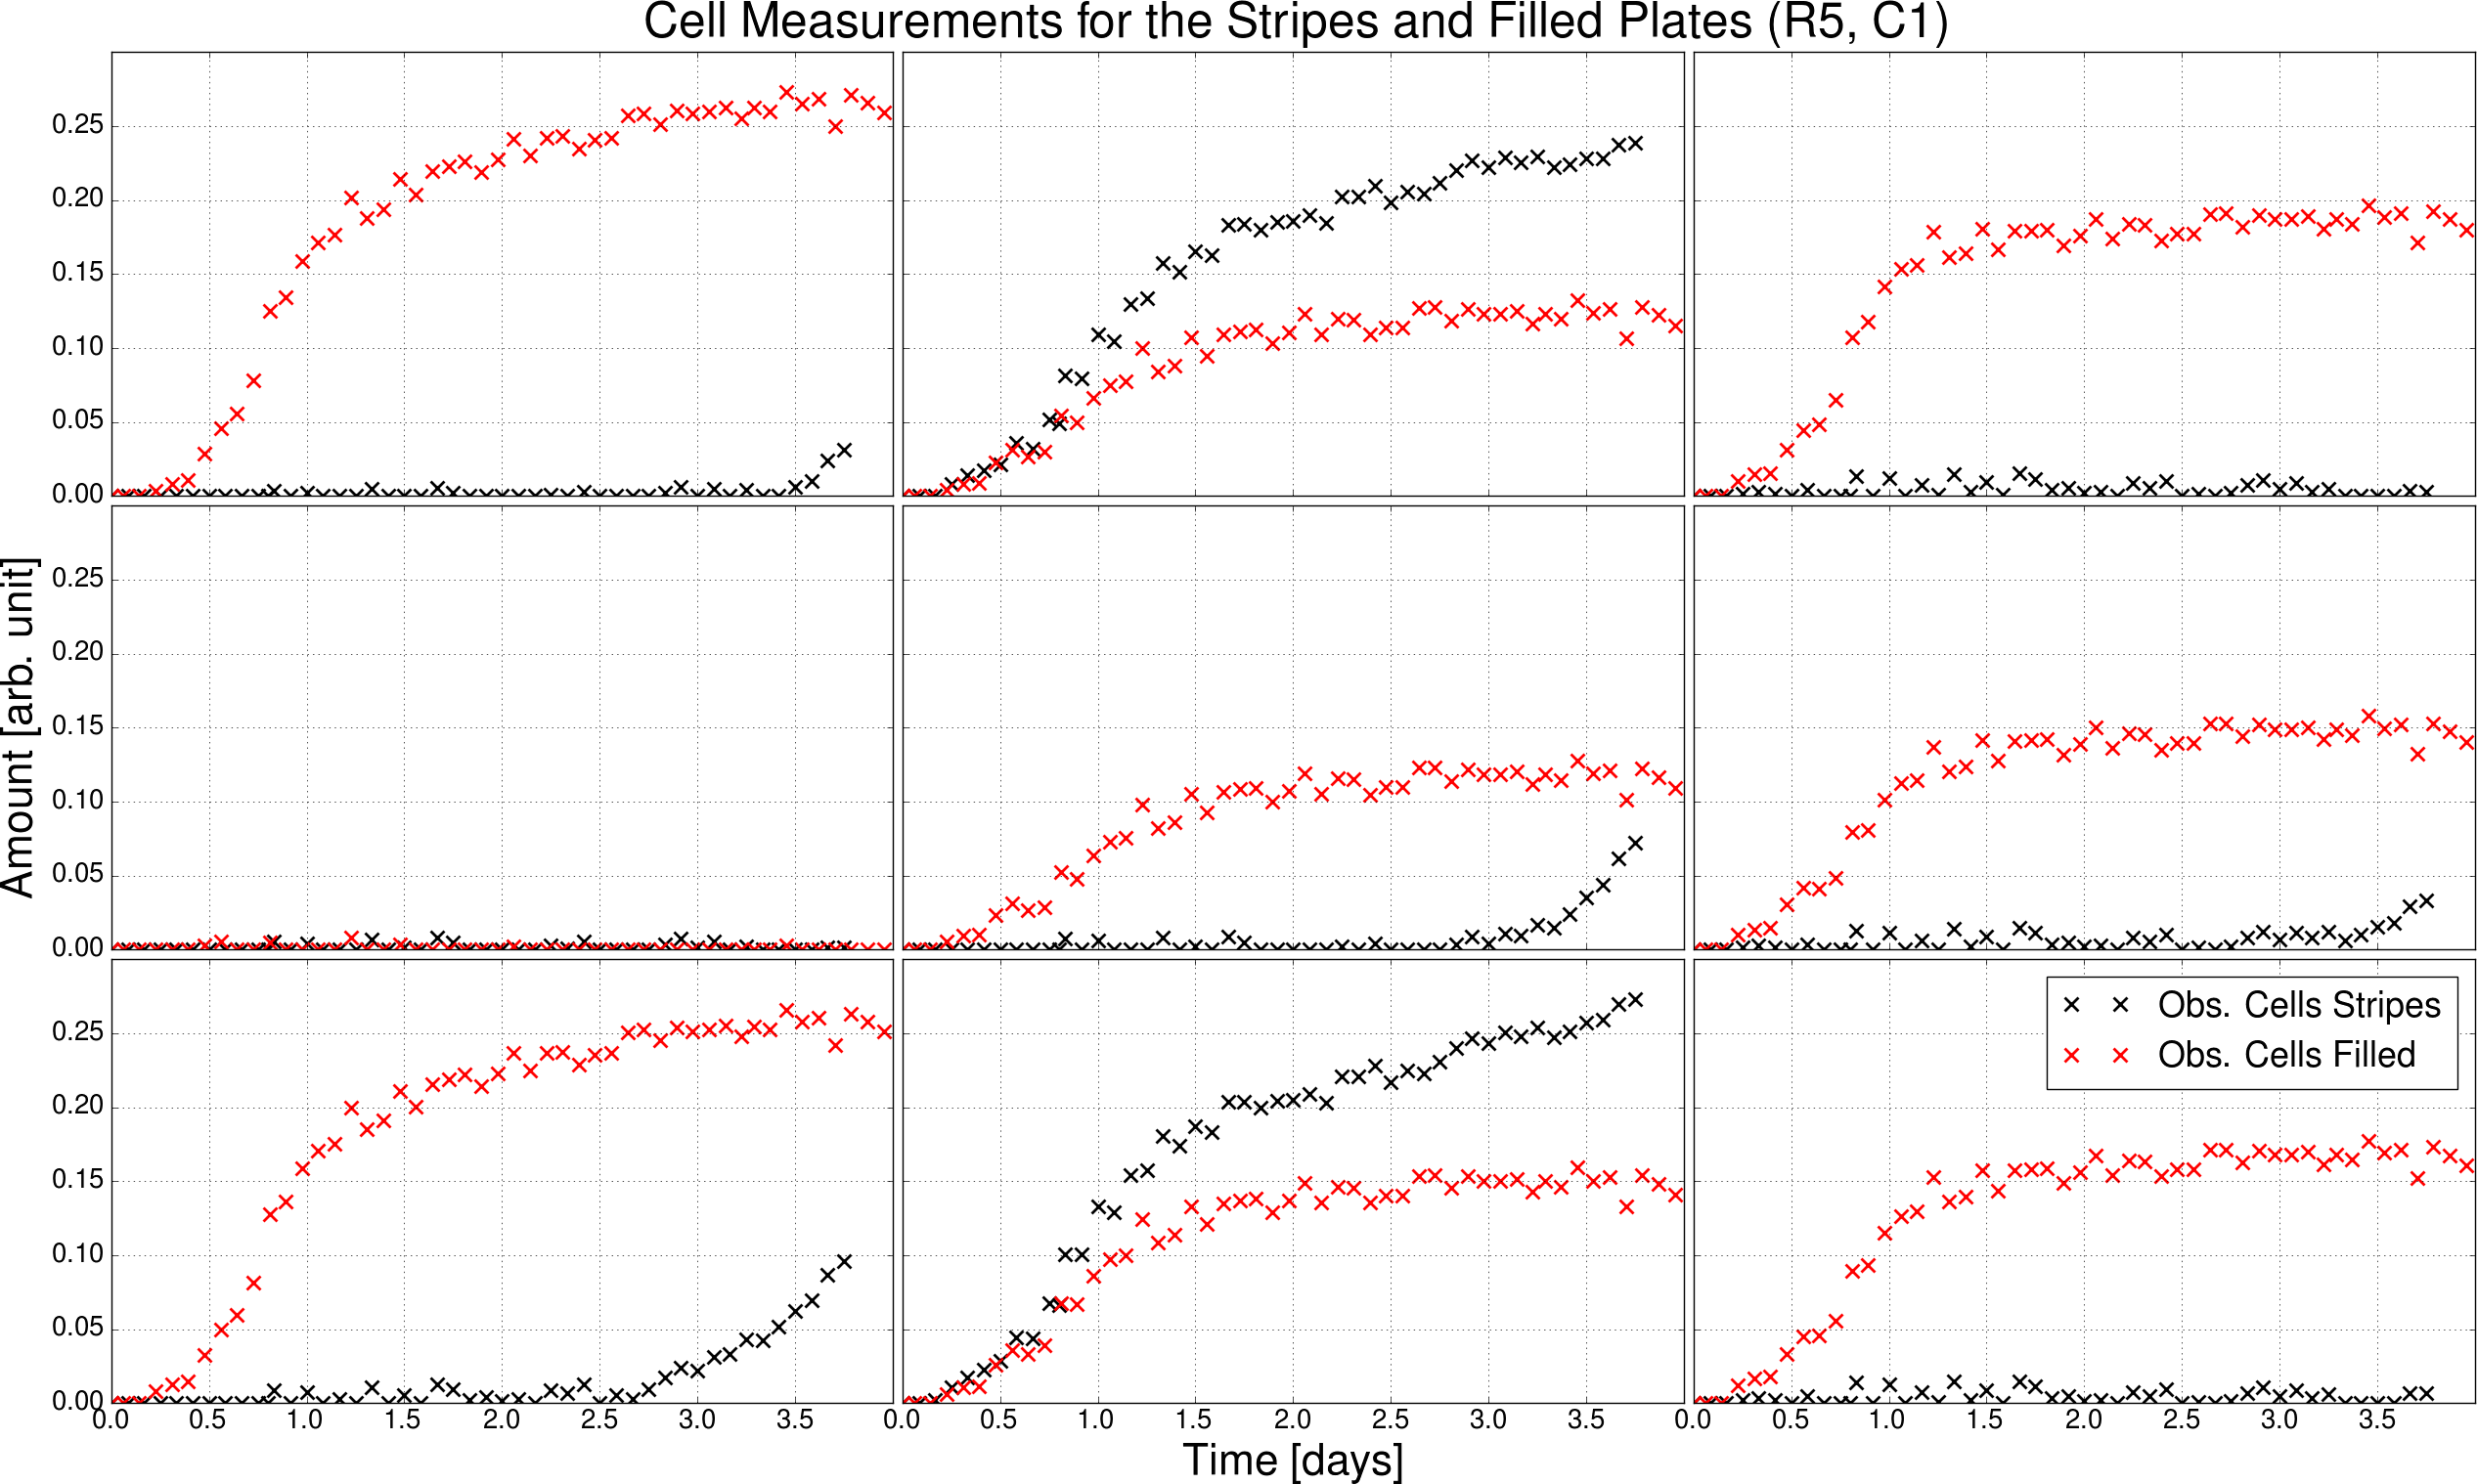
\includegraphics[width=\linewidth]{final/c_meas_r5_c1}
%   \captionof{figure}{Observed cells for (R5, C1) 3x3 zone of Stripes
%     and Filled plates showing (for Stripes data) slow growing cultures
%     starting to grow after faster growing cultures have reached the
%     stationary phase.}
%   \label{fig:kn_guessing}
% \end{Figure}


% We have only studied data where cultures are grown in an array on
% solid agar where we cannot validate the independent limit. In this
% limit, our model says that nutrients can only be converted to cells
% and all cultures starting with the same amount of nutrients will reach
% the same final cell density. This ignores metabolism which may differ
% between strains. Cell arrest could also limit growth (and this may
% occur in different strains at different rates). If present,
% differences in such effects could account entirely for differences in
% final cell density. However, they are unlikely to be the only effect,
% because this would not lead to the observed characteristic endpoint in
% growth. Using one-culture spot tests (in a perti-dish on ager?) or
% liquid cultures we can grow cultures independently and validate the
% independent limit. A current issue with methods for estimating
% fitness, is that identical strains grow differently on agar or in
% liquid culture leading to different fitness rankings (cite). This
% problem need not affect our validation as we can simply define a
% culture to have different parameters for growth in either medium. A
% greater difference may be caused by the dimensionality of the
% environment. Mass action kinetics is derived for reactions in a
% three-dimentsional (gas or fluid?) (Guldberg and Waage C.M. Guldberg
% and P. Waage, Studies Concerning Affinity, C. M. Forhandlinger:
% Videnskabs-Selskabet i Christiana (1864), 35) and this approximation
% is more valid for liquid cultures than for cultures spotted onto a
% surface. I suggest to study first the more ideal case of liquid
% cultures and later see if the model holds for cultures grown on a
% surface. If it does not, it may be necessary to use a fractal kinetics
% model (I have references for this from the proposal) or, if the
% reaction is diffusion limited, consider a more detailed model of
% nutrient diffusion.

% // Model equations for metabolism.//

% Our model splits the agar into a grid with volume discretised per
% culture. In the stripes validation, we overestimate the effect of
% diffusion when neighbouring cultures are removed. I believe that we
% are not accurately capturing the point at which growth becomes
% diffusion limited and that nutrients are well approximated as being
% evenly distributed withing the spatial scales that we model. A
% diffusion equation model could capture the local distribution of
% nutrients around a culture when the stationary phase is reached.  Reo
% and Korolev (2014) use the diffusion equation (with Neumann and
% Dirichlet boundary conditions) to simulate nutrient dependent growth
% of a single bacterial culture on a pertri dish in two-dimensions. They
% create a sink for nutrients from culture growth and equate the flux of
% nutrients through culture area with the rate of increase in culture
% size. They model culture area as varying and keep culture density
% constant. This model could be adapted for QFA by keeping culture area
% constant and allowing culture density to vary. A mass action kinetic
% model of reaction~(\ref{eq:reaction}) could be used for culture growth
% and the nutrient sink. Simulating or fitting this model could help us
% learn more about diffusion in QFA experiments. It is probably
% computationally unfeasible to use such a detailed model to fit a whole
% plate. However, if necessary, it may be possible to use a finer grid
% to increase compartmentalisation of nutrients to capture spatial
% heterogeneity in the distribution of nutrients around a culture and
% the effect of diffusion limited growth. This could extend the validity
% of the competition model over a larger range of variability in culture
% growth rates (for instance when some cultures are left empty and
% others are very fast growing.)

% It would also be useful to determine experimentally how nutrients are
% distributed throughout the agar at the stationary phase. Gaps could be
% left in an array of cultures and only inoculated once the stationary
% phase is reached. If they grow then nutrients remain. (Sill require
% simulations to see distribution across depth). This could be extended
% by growing a single column of identical strains and, after the
% stationary stage has been reached, inoculating identical strains on
% the same plate at different distances from the row.

% //Talk about an improvement to the imaginary neighbour model.//

% Nutrients (sugars, nitrogen, etc.) in QFQ agars are of a standard
% composition, designed to reduce the excess of any single nutrient
% (check QFA paper and cite). ((background) What is the nutrient?
% Nitrogen is only used to build molecules for new cells, whereas sugars
% are also used for metabolism.) For modelling nutrient limited growth,
% especially across plates, it would be useful to know the identity of
% the limiting nutrient and ensure that it is always the same. We could
% achieve this using a different formula of agar.

% The design of the stripes validation experiment could be
% improved. Rather than filling gaps with cultures not present on the
% stripes plate, and for which we have no b estimates, we could fill
% with repeats of the cultures already present on the stripes
% plate. (I'm not sure it makes any difference actually whether we
% validate from one direction to the other). It would also have been
% helpful to have repeats to study differences in COV between the
% competition and independent models. In order to make sure that
% competition effects were present in data, we made a drastic change
% between the stripes and filled plates. This provides a stern
% validation. The model assumes that competition effects are present
% whenever there is a difference in final cell amounts between
% cultures. We could have first validated the model against a smaller
% change, by varying between slower and faster growing cultures rather
% that none and very strong growing cultures. If the model works well
% between such plates it may work well for the majority of QFA
% experiments which typically have smaller differences between cultures
% than the data we study. If we did want to test the in an extreme case
% we could have inoculated fast growing cultures next certain strains
% and not others to try to induce a change in ranking for which the
% competition model might compensate better than the logistic model.

% //Signalling//

% If we find that competition for nutrients is not a significant effect,
% for instance if growth becomes diffusion limited before nutrients from
% neighbours can be accessed, then we could instead model signalling by
% ethanol as the interaction effect. This may be modelled similarly to
% how we are already modelling nutrient diffusion.

% //Signalling equation//

% If there is any combination of competition, metabolism, signalling, or
% arrest contributing significantly to differences in the growth of
% cultures and the interaction between neighbours then it will be
% difficult to separate them when fitting a model to data. We may have
% to develop ways to calibrate effects in isolation (e.g. by
% adding/measuring ethanol?) and use this information when fitting to
% high-throughput data.

% It is quicker to fit to small zones of a plate but as these have a
% larger proportion of edge cultures boundary conditions become
% important. In current data (e.g. P15), different cultures surround the
% edge and this makes accurate fitting difficult. As a result we must
% work with larger zones that take longer to analyse. We could surround
% small 3x3 and 4x4 zones with an empty ring and only need to consider
% net flux of nutrients across the boundary and not local variation due
% to different cultures surrounding the zone. We could also surround
% with the same, low-variance, strain to reduce net flux.
% % (Would it be better not to use a temperature dependent strain?)

% //Stochastic effects.//

% Unpublished work by Hermann and Lawless has investigated heterogeneity
% between cell lines within single QFA spots. They have found that a
% single or small number of extremely fast growing cell-lines come to
% dominate the population of a single culture. The implication is that
% cultures with a lower starting cell densities are likely to have
% greater variance between repeats. We could use higher starting cell
% concentrations to reduce this variance but then we study less of the
% growth phase. It may be possible to reduce heterogenetity by inoculating
% from the exponential growth phase rather than the stationary phase and
% still study full growth curves. (Unless mean population growth
% constant is being studied...) Staring cell densities should ideally be
% as close to the lowest resolvable level as possible.

% //Ways to measure \(C_{0}\)// There is a confounding effect between
% initial cell density and b value with may justify using initial cell
% densities slightly above the minimum detectable level. Hetoregeneity
% within cultures is an issue again here and cell density would
% effectively be lower than the measured value, e.g., if most inoculated
% cells are dead or slow growing.

% To fit growth curves more accurately QFA has begun using the
% generalised logistic model (cite). Fitness estimates (MDR*MDP or MDR?)
% from this model have higher coefficient of variation than those from
% either the standard logistic or competition model. (accuracy and
% precision? Could for instance a step function be less variable than
% the standard logistic model?)  Although the fits to data are
% qualitatively worse, it may be advisable to revert to the standard
% logistic model.


% The logistic model requires different K parameters (\(N_{0}\) for
% log. eq.) to be fit for each culture. The competition model shares
% information about \(N_{0}\) between cultures and therefore has 383
% fewer parameters for a full plate (Could this also explain the higher
% variance for the fastest growers?). For the slowest growing cultures,
% noise is more dominant and there is a confounding effect between r and
% K. To deal with this, the QFA R package uses heuristic checks. In the
% case of \textit{est1\(\Delta\)}, this has led to a dramatic
% disagreement in estimated fitness with the competition model. The
% estimate from (which model)? agrees better with existing biological
% knowledge (/independent spot experiments?). (Is the competition model
% then useful?)

% //QFA R is fixing \(C_{0}\) rather than fitting (I used a grid))//

% //Improvement to imaginary neighbour guessing//


%%% Local Variables:
%%% mode: latex
%%% TeX-master: "report"
%%% End:
